\chapter{Analysis}\label{chap:analysis}
    In this chapter, the general problem area of the danish people's concern about climate change, or the lack thereof, will be described. An apparent inconsistency between climate change awareness and the personal climate actions will also be investigated. Furthermore, the potential of transformative media platforms, particularly Immersive Virtual Reality(VR), as an approach for affecting real life behaviour, will be explored. The knowledge obtained throughout this chapter, will culminate in a set of design requirements and a problem statement that will be used to design, develop and evaluate upon a prototype of a VR experience with personal climate actions, meat consumption in particular, as the main theme.

\section{Problem Area}\label{sec:problemArea}
    For several years the consensus among scientists and the reliability of the scientific data regarding anthropogenic climate change, and predictions about future impact, has increased, making the issue hard to deny\cite{the5Ds, scientistConsensus, publicEngagementUnderstanding}. Around one third of many countries' carbon emission come from domestic energy-use and private travel\cite{reorientingClimageChangeCommunication}. There is, however, still a discrepancy between the public's awareness of the subject, in developed countries such as Denmark, and what individual people do to reduce their personal carbon footprint. Most of these people's lack of personal climate action, is a result of a psychological distancing towards the matter\cite{the5Ds, publicEngagementUnderstanding}. They believe that there will be no immediate personal consequences, because climate change is both spatially and temporally far away\cite{publicEngagementUnderstanding}.
    
    \subsection{Concito surveys}
        In a survey from 2018, made by the danish think tank Concito\footnote{\href{https://concito.dk}{Concito Website: https://concito.dk}}, respondents(n=1076) were asked about their opinions on climate change and their personal ${CO_2}$ footprint.
        
        The respondents were asked about how serious climate change was on a global scale. 46\% and 42\% responded with either very serious or to some degree, respectively. 
        
        When asked about to what degree they themselves were feeling the effects of climate changes, 4\% said that they were experiencing it to a great extent, while 21\% replied only to some extent. This leaves 44\% saying that they experienced it to a lesser degree and 24\% replying they did not experience at all\cite{concito}. This correlates with another question of the survey asking about how concerned the respondent were that climate change would personally hurt them, where 11\% said that they were greatly worried about damage to them, and 37\% replied that they were to some extent worried\cite{concito}.
        % Do not feel the effects
        
        When asked, 54\% said that they believe it is necessary for them to make behavioural lifestyle changes, while 24\% believe that technology will solve the climate issues, without them needing to make substantial lifestyle changes\cite{concito}.
        % About half feel a personal responsibility

        When it comes down to the expected climate action, the individual Dane does not make the required sacrifices to live up to their own expectations, with only 16\% saying they flew less from 2016-2018 and less than half(48\%) use the bike or public transportation. The question accepted multiple answers\cite{concito}.
        % People still fly a lot knowing that it is a "sin" only some people use bike or public transportation
        
        When asked about motives for making an effort towards more climate friendly measures like using public transport instead of a car, insulating their house post build, or buying less energy intensive appliances, only 30\% said that they did it to help the environment, while 31\% said they did it to save money. 23\% did however reply that they simply did not do those environmentally friendly efforts\cite{concito}.
        % There are about as many financially related incentives to change the individual behaviour than climate related
        
        In 2019 Concito released another report about the danish people's food consumption and the climate impact that follows, which was an updated version of a report they made in 2016. The reason for the update was that it has become a subject more in focus these last few years\cite{concitoFood}. The agriculture and forestry sector emits approximately 25\% of the global $CO_2$ emissions, and with an ever increasing world population, there is a need to reduce meat consumption and look into alternative plant based foods\cite{concitoFood}. According to Concito Denmark ranks number 13 of countries with the most meat consumption per citizen in the world\cite{concitoFood}.
        
        Based on this data, it seems that people in Denmark are well aware of climate change, and are concerned on a global scale. They do, however, not seem to feel the consequences of it themselves. Only about half of the respondents feel a personal responsibility to change their everyday behaviour, while the rest either believe in technology, none of the above or do not know. People are still flying as much as they used to, and only about half ride bikes or use public transportation and leave the car in the garage. It is not clearly described how many of the respondents actually own a car and how often they use it. The presented data from Concito confirms that there is a discrepancy between the level of awareness and the lack of personal action regarding the climate. Since Denmark is very high on the list of meat consuming countries, this is a good place to start as it is a specific area, within the vast subject of climate change, with a clear room for improvement.
    
    \subsection{5 Psychological Barriers}\label{sec:5barriers}
        The Norwegian Psychologist Per Espen Stoknes calls the discrepancy between awareness and action the \textit{psychological climate paradox}\cite{storyAboutClimateChange, the5Ds}. According to Stoknes, people tend to put up psychological barriers when confronted with climate change, and part of the reason is due to a failing communication about the subject. More specifically, he presents 5 psychological barriers(The 5 D's) that have to be broken down in order to achieve effective climate change communication. These are shown in \autoref{fig:5ds}.
        
        \begin{figure}[H]
        	\centering
        	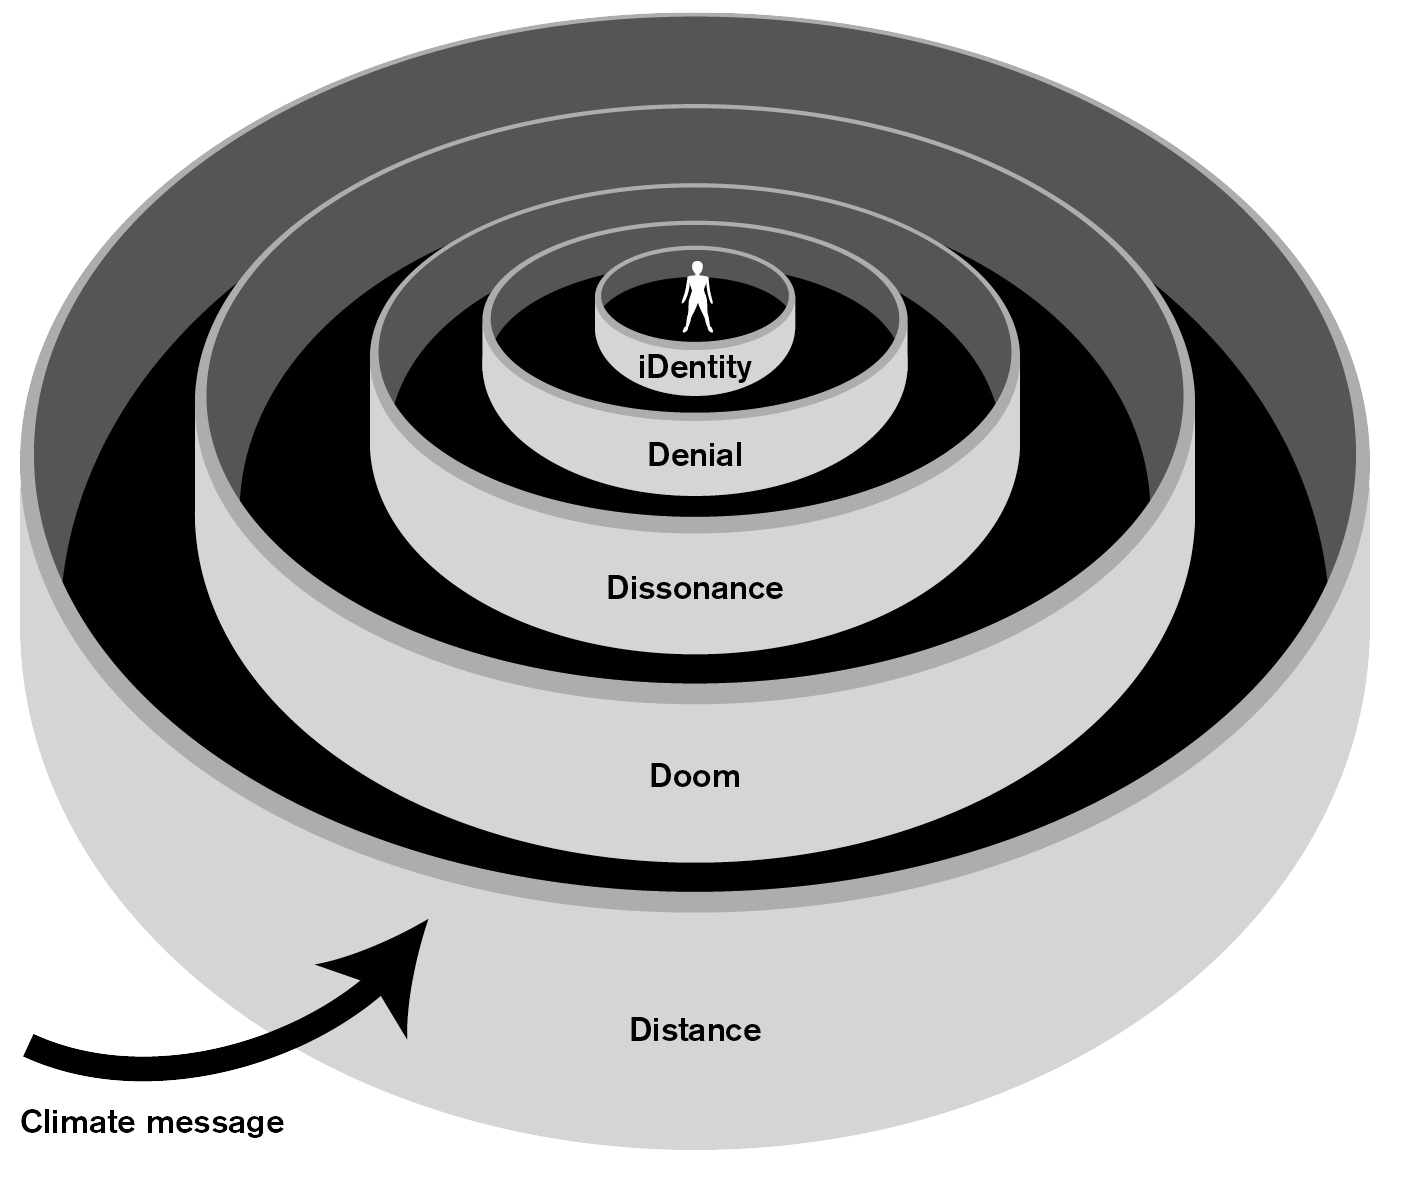
\includegraphics[width=0.9\linewidth]{figure/Analysis/5ds.png}
        	\captionsource{The five psychological barriers blocking the climate message}{What we think about when we try not to think about global warming - Per Espen Stoknes\cite{storyAboutClimateChange} (2015)}
        	\label{fig:5ds}
        \end{figure}
        
        The first barrier, \textit{Distance}, comes when exposed to e.g. a large amount of imagery of polar bears and melting ice in the mass media, which can feel remote and therefore unrelatable to a majority of people\citep[p.~108]{storyAboutClimateChange}. In order to break it the communication needs to feel near, personal and urgent\cite{the5Ds}.
        The second barrier, \textit{Doom}, arises through fear messaging. When the climate change is framed as an inevitable disaster or the end of the world, people have a tendency to become disengaged and avoid the topic altogether\citep[p.~109]{storyAboutClimateChange}. This way of communicating should be replaced with a more positively framed communication as fear is not a good motivator. Instead of looking at climate change as a only a disaster, look at it as an opportunity for green growth and a healthier life due to the replacement of meat with vegetables\cite{the5Ds}.
        \textit{Dissonance} occurs when the knowledge about e.g. the usage of fossil fuels or the meat consumption, does not match peoples behaviour. They will still drive cars and fly on vacation and eat meat. It is easy to fall in the trap of self-justification when comparing one self to other people who eat even more meat or drive and fly everywhere\citep[p.~109]{storyAboutClimateChange}. By making it simple to do the right thing, this barrier could be avoided. An example of this is a hotel that reduced their plate sizes and thereby reduced their food waste by approximately 20\%\cite{the5Ds}.
        \textit{Denial} is a self-defence mechanism that happens despite the amount of information and the individual's intelligence\citep[p.~109]{storyAboutClimateChange}. If something is too incomprehensible to the ego a new reality will be manufactured and believed. A positive narrative, avoiding denial triggering emotions, such as anxiety, guilt, fear and shame, but instead tells stories about heroes fighting destruction and good news about new scientific findings etc.\cite{the5Ds}.
        \textit{Identity} is the inner most barrier. The cultural or political identity of a person can determine whether or not a person is willing to accept and adapt to climate messaging\citep[p.~109]{storyAboutClimateChange}. Networking in the local communities can help bypass this barrier, as it is a powerful tool to inspire others and reducing the cultural and political division on the subject matter\citep[p.~133]{storyAboutClimateChange}\cite{the5Ds}.
        
        When these barriers have been broken down, using positive strategies, a successful communication about climate change has been achieved, there will be an increase in the perceived importance of the issue and the public will get more engaged in personal climate action\cite{the5Ds}. It is argued that engagement consists of 3 parts. There has to be an \textbf{understanding} of the urgency of the subject at hand. There has to be an \textbf{emotional} connection, which raises concern to it and there has to be a consistent \textbf{behaviour}\cite{climateChangeEngagement3Elements, vrEngagementClimateChange, reorientingClimageChangeCommunication}. The lack of personal action towards a more cleaner environment is a problem that needs attention in Denmark. In order to make the public engaged in the climate, a more positive communication has to take place. As Per Stoknes says: 
        \begin{quote}
            \textit{We’re in this for the long haul. Why not make it enjoyable, meaningful, funny, enriching?}\citep[p.~117]{storyAboutClimateChange}
        \end{quote}
        
        
\section{Behavior change}
    As concluded in the previous section the problem is that the danish people's behaviour does not match the knowledge and concern they have. This is due to the failed climate communication on the issue(See \autoref{sec:5barriers}). Therefore, research on how to change a behaviour without triggering psychological defence mechanisms seems appropriate.
    This section describes how games can be used as a tool to transform people's worldview and thereby incite a behaviour change. It describes an "\textit{embedded design model}" and how it can be applied to a game to avoid raising the players' psychological barriers when tackling a serious issue. 
    Furthermore, it explores how Immersive Virtual Reality(VR) and the potential of Immersive Virtual Environments(IVE) also can be used to transform and change real world attitudes or behaviours towards a given subject.
    
   \subsection{The embedded design model}
    Games can be used as more than just entertainment and to pass time. Transformative or persuasive games can be developed with a greater purpose\cite{transformationalFramework}. They can present players with complex societal issues, which could lead to a change in perspective and ultimately an increased climate engagement and change in their behaviour\cite{persuasiveGameplay}. A lot of these types of persuasive games do, however, tend to fall into the trap mentioned in \autoref{sec:5barriers} of being to literal in their message, and thereby raising psychological barriers\cite{embeddedDesignModel}.
    
    The embedded design model, proposed by Kaufman et al., is a way to avoid raising these psychological barriers, when dealing with serious issues in games\cite{embeddedDesignModel}. In order to not be forceful and use fear messaging(see \autoref{sec:5barriers}) when communicating about climate change this "\textit{embedded model}" should be considered\cite{embeddedDesignModel}. The model consists of 3 primary strategies, that are all methods of embedding serious topics into games and making them less direct. These strategies are shown in the list below:
    \begin{itemize}
        \item Intermixing
        \item Obfuscating
        \item Distancing
    \end{itemize}
    
    \textbf{Intermixing} means that the serious messages of a game is mixed in with unrelated ones to avoid the users feeling overloaded with the games serious content\cite{embeddedDesignModel}. Tests, comparing an overloaded version of a game with an intermixed version, have shown that an intermixed version invites a more open mindset and is more likely to circumvent psychological barriers\cite{embeddedDesignModel}. According to Kaufman et al. the ideal ratio of on-message and off-message is approximately $45\%/55\%$ respectively. This was tested against an overloaded ratio of $75\%/25\%$.\\
    \textbf{Obfuscating} is about diverting the attention from the serious intent through framing devices such as an unexpected choice of genre or delaying the revelation of the actual message of the game\cite{embeddedDesignModel}.\\
    \textbf{Distancing} uses metaphors and hypothetical scenarios to embed the message of the game. An example of this is is a game about vaccination. Instead of using what is directly relatable to the players, the message is covered up with a zombie theme instead\cite{embeddedDesignModel}.
    
    These strategies can either all be applied in one game, or one or more of them can be picked individually, and have shown positive result during tests\cite{embeddedDesignModel, embeddedDesignModelTestDetails}. Kaufman et al. has tested the model on physical non-digital board games and card games, but encourages the implementation of embedded design across various digital media platforms as well\cite{embeddedDesignModel}. One of the mediums that has also shown a great potential in this field is VR\cite{persuasiveGameplay, vrCapabilitiesSlater}.
    % Encourages to implemented and test on other digital media
    
    \subsection{Transformation through experiences in VR}
    VR experiences also have the ability to place people in environments otherwise inaccessible to them\cite{vrCapabilitiesSlater, emotiveImagery} and thereby give them an transformative experience that could potentially change their worldview and behaviour in the real world\cite{transformativeVR, riva2016transforming}. Due to the substitution of sensory input that VR is capable of, primarily visual and auditory, a user's perception of these inputs are interpreted the same way in the brain as inputs in reality, even though the user is fully aware of the virtual world\cite{vrCapabilitiesSlater}. Through VR a user can experience a sense of presence that is an effective tool for personal change\cite{riva2016transforming}. Furthermore, the virtual environment can also bring out emotional responses that can lead to behaviour change\cite{transformativeVR, ahn2011embodied}.
    
    Climate change engagement can be furthered through the Immersive Virtual Environments (IVE) experienced through VR\cite{vrEngagementClimateChange}. IVEs are good way of facilitating a more conceptual understanding of complex issues in a comprehensible way through visual and auditory stimuli. The imagery presented through VR can provide a visualisation of how the future could look if the current behaviour is not changed\cite{emotiveImagery}. It is, however, also in VR, important not to trigger disturbing feelings and feelings of unease if the imagery is supposed to be motivating and engaging, as this will raise defensive psychological barriers\cite{emotiveImagery}.
    
    According to E. Stepanova et al., going from a perceptual experience in VR to a cognitive shift and finally to behaviour change requires specific transitions to happen\cite{transformativeVR}. A perceptual experience needs to fall outside the current worldview of the user, creating a perceptual dissonance, and only by changing the worldview one can accommodate for the new perspectives, which would lead to a cognitive shift. From this cognitive shift a conflict will arise between the new world view and the current, still unchanged, behaviour. In order for this conflict to be resolved either the new worldview has to be rejected or the behaviour need to change\cite{transformativeVR}.
    
    \subsection{Immersive Virtual Environments (IVE)}
    Understanding: More conceptual understanding of complex issues\cite{vrEngagementClimateChange}
    Emotion: Potential to elicit emotional states through manipulating the visual, auditory and haptic stimuli presented to the user
    Behavior: Embodied cognition. We interact, communicate and learn through movements, gesture and physical activities

    
    \subsubsection{Sub-conclusion}
    Games on the subject of climate change are well-suited to address climate challenges because they can serve as effective tools for education and engagement\cite{gamesAsToolsForEngagement}
    The embedded model should be used to get the message across and lower the psychological barriers that arise when a serious social issue is communicated too directly and forthright(see \autoref{sec:problemArea})
    IVE's are effective visualisations tools to communicate complex issues.
    Transformative experiences are more accessible through VR


\section{Immersive virtual Reality}
    Virtual Reality could be used to effectively communicate about climate change. 
    The strength of the emotion(see \autoref{sec:problemArea}) is linked with the users sense of presence\cite{vrEngagementClimateChange}
    
    \subsection{Presence}
    "Newer forms of digital media such as video games or virtual reality simulation are particularly more likely to result in high presence compared to traditional media"\cite{ahn2011embodied}.
    
    Place Illusion (PI) is the type of presence that refers to the sense of "being there"\citep{vrImmersion}[p.~3551].
    
    Plausibility Illusion (Psi) is the illusion that what is perceived to be happening is actually happening\citep{vrImmersion}[p.~3553].
    
    The Plausibility Illusion does not not require realistic appearances, nor does it require realistic behaviour\citep{vrImmersion}[p.~3553]. In the control condition from Slater's paper, the virtual object simply had a humanoidal look, but could not be mistaken for a human in neither movements nor appearance\citep{vrImmersion}[p.~3553].
    
    The body is where PI and Psi are combined, and is instrumental in providing evidence for PI\citep{vrImmersion}[p.~3554]. When looking down at your body, wearing a HMD(Head Mounted Display), and seeing your body in the place that you expected provides strong evidence for PI\citep{vrImmersion}[p.~3554].
    
    You know that this virtual body is not yours, but simply a representation\citep{vrImmersion}[p.~3554]. When moving your body and seeing the limbs move accordingly, also provides a connection between the visual external world and the user\citep{vrImmersion}[p.~3554].
    
    \subsubsection{Sub-conclusion}
    By invoking a sense of presence, IVEs can support intense feelings that make a user think, feel and behave as though they are really embedded in the place represented by the computer generated virtual space.
    By not breaking place illusion and plausability illusion a user will feel presence
    
    
\section{State of the art}
    \subsection{Water consumption}
    Exaggerated ambient feedback has proved to have a positive effect.\cite{waterConsumption}


\section{FPS}\label{sec:FPS}
\begin{quote}
    How can Intermixing
    How can an immersive virtual reality transformational game incite an intent of behavioural change towards personal climate action in regards to $CO_{2}$ emissions? \todo{Tack on behavior change theory}
\end{quote}

\section{Design Requirements}\label{designReq}

\subsection{Functional design requirements}
% Make cites into refs for sub conclusions for each section.
\begin{itemize}
    \item Should incite an intent for a personal behaviour change in regards to CO$_2$ emissions.\todo{SPECIFY theory}
    \item Should implement immersive Virtual Reality to increase a sense of presence and engagement.
    \item Should lower psychological barriers, in regards to CO$_2$ emission believes.\cite{the5Ds}
    \begin{itemize}
        \item Distant
        \item Doom
        \item Dissonance
        \item Denial
        \item iDentity
    \end{itemize}
\end{itemize}


\subsection{Non-functional design requirements}
\begin{itemize}
    %Behavior change
    \item Use the transformational framework to incite behavioural change.\cite{transformationalFramework}
    %Water Consumption
    \item Use ambient exaggerated feedback(AEF) to incite a behaviour change \cite{waterConsumption}
    
    % VR
    \item Should try to maintain high Place Illusion (PI), for Immersion\citep{vrImmersion}[p.~3551].
    \item The virtual environment should be non realistic, to reduce the amount of PI breaks.
    \item Should have a virtual body to increase evidence for Plausibility Illusion(Psi), for believability \citep{vrImmersion}[p.~3553].

    %Narrative
    \item Use the player engagement process model to create engagement, incite emotions, and provide an engaging story\cite{playerEngagement}.
    %\item The narrative should challenge previous knowledge of the player, to create an engaging story.%Where is this from?
    %\item Use supportive framing that do not backfire by creating negative feelings.%Where is this from?
    
    %Embedded model
    \item It should make use of the \textit{Embedded design model} to lower psychological defences that arise when a serious social issue is communicated too directly and forthright\cite{embeddedDesignModel}.
    
    %5Ds
    \item Make the issue feel near, human, personal, and urgent to lower the distance barrier %Distance
    \item The narrative should make use of a positive story, to lower the doomsday barrier. %Doom
    \item Reduce dissonance by providing opportunities for consistent and visible action.\todo{Needs to be rephrased} %Dissonance
    \item Avoid triggering the emotional need for denial through fear, guilt, self-protection\cite{the5Ds}. %Denial
    %We need an identity requirement, if possible
    
\end{itemize}